\documentclass[11pt,titlepage,fleqn]{article}

\usepackage{amsmath}
\usepackage{amssymb}
\usepackage{latexsym}
\usepackage[round]{natbib}
\usepackage{xspace}
\usepackage{graphicx}
\usepackage{epstopdf}
%\usepackage{epsfig}

\usepackage{pifont}   % search for \ding

%\usepackage{fancyhdr}
%\pagestyle{fancy}

%=====================================================
%       SPACING COMMANDS (Latex Companion, p. 52)
%=====================================================

\usepackage{setspace}

%---------------------------
\newcommand{\matlab}{\textsc{Matlab}\xspace}
%---------------------------
\renewcommand{\baselinestretch}{1.0}

\textwidth 460pt
\textheight 700pt
\oddsidemargin 0pt
\evensidemargin 0pt

% see Latex Companion, p. 85
\voffset     -50pt
\topmargin     0pt
\headsep      20pt
\headheight    0pt
\footskip     30pt
\hoffset       0pt

\include{carlcommands}
%\input{dp_header}

\graphicspath{
  {/home/vipul/REPOSITORIES/IITR_seismo/classes/ES510/latex/figures/}
  }

\begin{document}

\noindent Course: Numerical Methods and Computer Programming\\
\noindent Code: ES 510\\
\noindent Instructor: Vipul Silwal (\verb+vsilwalfes@iitr.ac.in+) \\ 
\noindent Last Compiled: \today \\

{\huge Basics of probability}

\verb+ textbook: Inverse Problem Theory by Albert Tarantola+
\tableofcontents
%% ------------------------------------------------------------------------ %%

\begin{section}{Introduction}
The probability of occurrence of an event $A$ is represented by $P(A)$; $A$ is a subset of all the possible events in the domain $X$, $A \subseteq X$. $A$ could be a point, a subset of points, or a continuous function. There always exists some function $f(\pmb{x})$ through which we can obtain the probability $P$ over $A$.

\begin{equation}
P(A) = \int_A d\pmb{x} f(\pmb{x})
\end{equation}
where 
\begin{equation}
\int_A d\pmb{x} = \int dx_1 \int dx_2 ...
\end{equation}
where $d\pmb{x} = \{x_1, x_2, ....\}$ are the independent model parameters (or the dimensions of the system, or the coordinate system).
\\
\\
{\bf Model space}

In modelling, {\it model parameters} refers to a set of independent parameters that can explain the system. The number of independent model parameters is called dimensionality of the system. 
For example, in gravitation equation
\begin{equation}
g = \frac{GM_1M_2}{r} \label{grav}
\end{equation}
$\{M_1,M_2,r\}$ are the model parameters and the dimensionality is 3. In this case, $G$ is the gravitational constant and not a variable.

The possible range of values that the model parameters can take is termed as model space $M$. This model space could be discretized into individual model points. $M = \{m_1,m_2.....m_N\}$ (not the same $m_1,m_2$ as in equation \ref{grav}). Then each model point would be:

\begin{eqnarray*}
m_1 &=& \{M_{11}, M_{21}, r_1\}\\
m_2 &=& \{M_{12}, M_{22}, r_2\}\\
&:&\\
m_N &=& \{M_{1N}, M_{2N}, r_N\}
\end{eqnarray*}

\fbox{\begin{minipage}{15cm}
 Example 1.3 from \cite{Tarantola2005}: Let's characterize the bulk modulus and the shear modulus, $\{m_1,m_2\} = \{\kappa,\mu\}$. A definition of the distance between two elastic media is:
\begin{equation}
d = \sqrt{(\log\frac{\kappa_2}{\kappa_1})^2 + (\log\frac{\mu_2}{\mu_1})^2}
\end{equation}
This clearly shows that the two coordinates $\{m_1,m_2\} = \{\kappa,\mu\}$ are
not Cartesian (rectangular).  Introducing the logarithmic bulk modulus $\kappa^* = \log\frac{\kappa}{\kappa_0}$ and the logarithmic shear modulus $\mu^* = \log\frac{\mu}{\mu_0}$ (where $\kappa_0$ and $\mu_0$ are arbitrary constants) gives
\begin{equation}
d = \sqrt{(\kappa_2^* - \kappa_1^*)^2 + (\mu_2^* - \mu_1^*)^2}
\end{equation}
The logarithmic bulk modulus and the logarithmic shear modulus are Cartesian coordinates over the model space $M$.
\end{minipage}
}
\\
\\
\\
{\bf Data space}

The observations during a physical experiment form the data space. $D=\{d_1,d_2...d_N\}$.

In equation $\bd = \bG \bem$, $\bG$ is the constitutive equation that maps model space $\bem$ to data space $\bd$.
\end{section}

%-----------------------------------------------------

\begin{section}{Homogeneous Probability Distribution and Likelihood}
Homogeneous Probability distribution means that probability of occurence of event in any subset $A$ of the entire space $X$, where $A \subseteq X$, is equal everywhere.
\\

\begin{tabular}{c|cc}
homogeneous box &
homogeneous sphere ({\it incorrect}) &
homogeneous sphere ({\it correct}) \\
\hspace{-2.5cm}
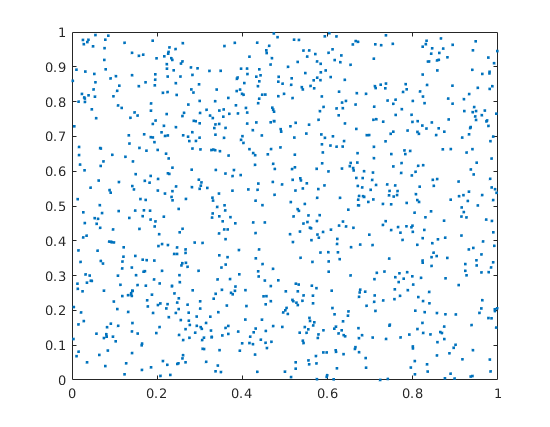
\includegraphics[scale=0.45]{homo_box.png} &
\hspace{-1.cm}
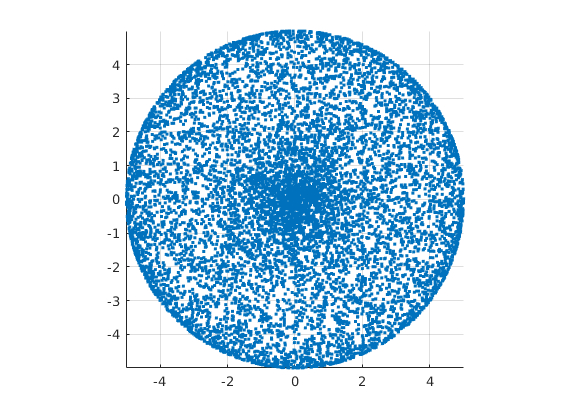
\includegraphics[scale=0.5]{homo_sphere_incorrect.png} &
\hspace{-1.75cm}
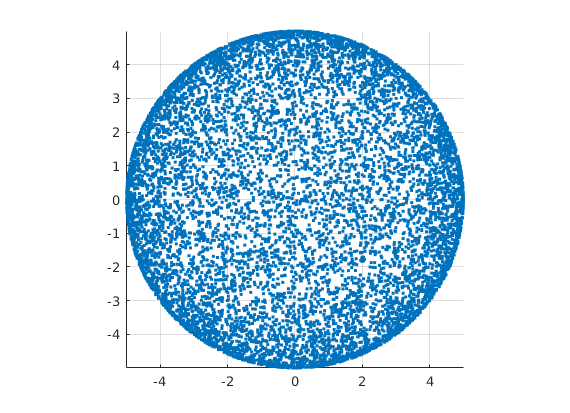
\includegraphics[scale=0.5]{homo_sphere_correct.png} \\
\end{tabular}

If $f(\bx)$ is a probability density and $\mu(\bx)$ is the homogeneous probability density, the ratio gives us the likelihood of the event (or the {\it volumetric probability}).
\begin{equation}
\phi(\bx) = \frac{f(\bx)}{\mu(\bx)}
\end{equation}


{\bf Disjunction and Conjuction of Probability Distributions}
Disjunction of two probability distributions could be thought of as the OR function; whereas the conjuction of the probability distributions could be thought of as the AND function.

\underline{Disjunction:}
\begin{equation}
(f_1 \vee f_2)(\bx) = \frac{1}{2}(f_1(\bx) + f_2(\bx))
\end{equation}

\underline{Conjunction:}
\begin{equation}
\frac{(f_1 \wedge f_2 \wedge \cdots \wedge  f_n)(\bx)}{\mu(\bx)} = \frac{1}{\nu} \frac{f_1(\bx)}{\mu(\bx)} \frac{f_2(\bx)}{\mu(\bx)} \cdots \frac{f_n(\bx)}{\mu(\bx)}
\end{equation}
where $\mu(\bx)$ is the homogeneous probability distribution in space $X$ (or the manifold $X$), and $\nu = \int_X \frac{1}{\nu} \frac{f_1(\bx)}{\mu(\bx)} \frac{f_2(\bx)}{\mu(\bx)} \cdots \frac{f_n(\bx)}{\mu(\bx)}$ is the normalization constant.

\end{section}
%-----------------------------------------------------

\begin{section}{Bayesian}
{\bf Conditional probability}
Conditional probability is the probability of occurence of an event $A$ given a prior event $B$ has already taken place.
\begin{equation}
P(A|B) = \frac{P(A \cap B)}{P(B)} \label{bayes1}
\end{equation}

Bayesian theorem provides a relation between $P(A|B)$ and $P(B|A)$. In geophysics, $A$ and $B$ and typically model parameters and observed data. The theorem is useful in answering the question: `what is the probability that my obtained model (parameters) is correct given the probability of fit for observed data is so and so'.
In later section we will see how probability could be obtained from misfit between the modeled data and observed data.
\begin{equation}
P(B|A) = \frac{P(A \cap B)}{P(A)} \label{bayes2}
\end{equation}

Equating both sides of equations \ref{bayes1} and \ref{bayes2}
\begin{eqnarray}
P(A|B) P(B) &=& P(B|A) P(A) \\
P(A|B) &=& \frac{ P(B|A) P(A) }{P(B)}
\end{eqnarray}

\end{section}
%-----------------------------------------------------

\begin{section}{Normal distribution}

\begin{equation}
f(x|\mu,\sigma^2) = \frac{1}{\sqrt{2 \pi \sigma^2}} e ^{-\frac{(x - \mu)^2}{2 \sigma^2}}
\end{equation}
where $\mu$ is the mean or expectation of the distribution and $\sigma$ is the standard deviation ($\sigma^2$ is the variance).

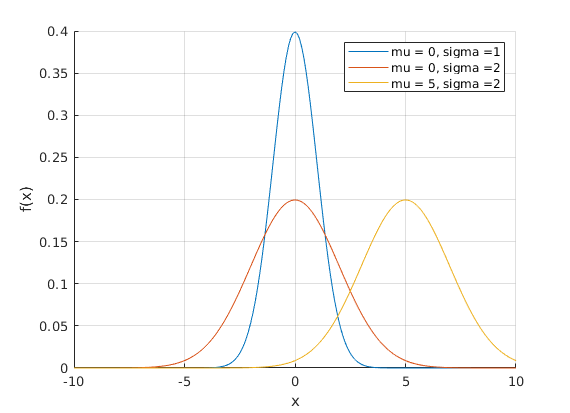
\includegraphics[scale=0.75]{normal_distribution.png}

Normal distributions (or gaussian distribution) are the most commonly used statistical distribution which assumes that

From geophysical perspective, this means that the {\it observed data} is normally distributed around the {\it actual} observed data. This discrepancy comes from the noise (from known and unknown sources) in the system. Even though this is a common assumption there is no (not much) scientific reasoning behind {\it why error should be normally distributed} (and not skewed gaussian or some other distribution). Later in the class we will see that least square solution are obtained under the assumption of normally distributed errors.
\end{section}
%-----------------------------------------------------

\begin{section}{Example}
{\bf Objective:} Compute probability from misfit between observed data and modelled data. 

\end{section}
%-----------------------------------------------------

\begin{section}{Exercise}

\begin{enumerate}

\item Two dimensional gaussian function is represented by:
\begin{equation}
f(x,y) = A \exp \left( - \left ( \frac{(x - x_0)^2}{2\sigma^2_x} + \frac{(y - y_0)^2}{2\sigma^2_y} \right ) \right )
\end{equation}
where $A$ is the normalization coefficient.

Write the formula for $A$ and estimate its value for the case: $x_0 = y_0 = 0$ and $\sigma_x = \sigma_y = 1$. Compute and plot the results.
\end{enumerate}
\end{section}

\bibliographystyle{agu08}
\bibliography{carl_main}
\end{document}
